\documentclass[12pt,a4paper]{article}
\usepackage[utf8]{inputenc}
\usepackage[T5]{fontenc}
\usepackage[vietnamese]{babel}
\usepackage{amsmath, amssymb, mathtools}
\usepackage{graphicx}
\usepackage{float}
\usepackage{geometry}
\geometry{a4paper, margin=2.5cm}
\usepackage{xcolor}
\usepackage{fancyhdr}
\usepackage{enumitem}
\usepackage{caption}
\usepackage{needspace}
\graphicspath{{img/}}
\usepackage{tikz}
\usetikzlibrary{shapes.geometric, arrows.meta, calc, positioning, babel}
\usepackage[hidelinks]{hyperref}

\newcommand{\nguoiA}{Nguyễn Đức Hiếu - 2410997}
\newcommand{\nguoiB}{Đào Ngọc Thanh Tú - 2413841}
\newcommand{\ngaynop}{16/11/2026}

\pagestyle{fancy}
\setlength{\headheight}{15pt}
\fancyhf{}
\fancyhead[L]{Xử Lý tín hiệu số}
\fancyhead[C]{HK261}
\fancyhead[R]{CO2036}
\fancyfoot[C]{\thepage}
\renewcommand{\headrulewidth}{0pt}

\setlength{\parindent}{0pt}
\setlength{\parskip}{4pt}

\begin{document}

\begin{center}
\vspace*{3.5cm}
{\LARGE BÀI THỰC HÀNH XỬ LÝ TÍN HIỆU SỐ\par}
\vspace{1.2cm}
{\LARGE LAB 5\par}
\vspace{1.2cm}
{\large \nguoiA\par}
{\large \nguoiB\par}
{\large \ngaynop\par}
\end{center}
\newpage

\section*{Tổng Quan}
Báo cáo trình bày kết quả Lab 5 môn Xử lý tín hiệu số về biến đổi $Z$, biến đổi $Z$ một phía ($Z^{+}$) và biến đổi $Z$ ngược. Nhóm giải 6 bài Exercise trong tài liệu hướng dẫn và 8 bài tập thêm của Chương 3 (Proakis): 3.3, 3.4, 3.7, 3.8, 3.13, 3.14, 3.19, 3.20. Với mỗi bài, báo cáo nêu tính chất hoặc cặp biến đổi được dùng, các bước biến đổi, kết quả và miền hội tụ (ROC); nhiều kết quả được kiểm tra lại bằng phương trình sai phân hoặc bằng giá trị đầu. Các bài Exercise 2, 4, 6 và Bài 3.4, 3.20 có thêm phần kiểm chứng bằng Scilab 2026.1.0.

\begin{table}[H]
\centering
\begin{tabular}{|l|l|}
\hline
\textbf{Thành viên} & \textbf{Phần việc} \\ \hline
\nguoiA & Exercise 1, 2, 4, 6; Bài 3.3, 3.4, 3.20 \\ \hline
\nguoiB & Exercise 3, 5; Bài 3.7, 3.8, 3.13, 3.14, 3.19 \\ \hline
\end{tabular}
\end{table}

\section*{1. Giới Thiệu}
Biến đổi $Z$ biến phép tích chập trong miền thời gian thành phép nhân trong miền $z$ và biến phương trình sai phân thành phương trình đại số. Vì vậy nó là công cụ chính để tìm đáp ứng xung, đáp ứng của hệ LTI với một ngõ vào cho trước, và để đánh giá tính nhân quả, ổn định qua vị trí cực và ROC. Biến đổi $Z$ một phía cho phép giải phương trình sai phân có điều kiện đầu khác 0, tách đáp ứng thành đáp ứng không vào $y_{zi}(n)$ và đáp ứng trạng thái không $y_{zs}(n)$.

\section*{2. Mục Tiêu}
\begin{itemize}
    \item Tìm biến đổi $Z$ và ROC của các tín hiệu một phía, hai phía; vận dụng các tính chất tuyến tính, dịch thời gian, đảo thời gian, tích chập, đạo hàm, liên hợp phức và co giãn trong miền $z$.
    \item Tìm biến đổi $Z$ ngược bằng khai triển phân thức tối giản, xét đủ các trường hợp ROC (nhân quả, phản nhân quả, hai phía).
    \item Tìm đáp ứng xung, đáp ứng không vào và đáp ứng trạng thái không của hệ LTI mô tả bằng phương trình sai phân; vẽ sơ đồ khối của hệ.
    \item Đọc và lập $X(z)$ từ giản đồ cực -- không.
\end{itemize}

\section*{3. Phương Pháp}
Biến đổi $Z$ hai phía và một phía:
\[
X(z)=\sum_{n=-\infty}^{\infty}x(n)z^{-n},\qquad X^{+}(z)=\sum_{n=0}^{\infty}x(n)z^{-n}.
\]
Các tính chất và cặp biến đổi chính:
\begin{itemize}
    \item Dịch thời gian: $x(n-k)\leftrightarrow z^{-k}X(z)$. Với $Z^{+}$, điều kiện đầu được đưa vào phương trình qua
    \[ x(n-k)\leftrightarrow z^{-k}\Big[X^{+}(z)+\sum_{n=1}^{k}x(-n)z^{n}\Big],\quad k>0. \]
    \item Tích chập: $x_1(n)*x_2(n)\leftrightarrow X_1(z)X_2(z)$. Đạo hàm: $n\,x(n)\leftrightarrow -z\,\dfrac{dX(z)}{dz}$. Đảo thời gian: $x(-n)\leftrightarrow X(z^{-1})$.
    \item $a^nu(n)\leftrightarrow\dfrac{1}{1-az^{-1}}$, $|z|>|a|$; \quad $-a^nu(-n-1)\leftrightarrow\dfrac{1}{1-az^{-1}}$, $|z|<|a|$.
    \item $(n+1)a^nu(n)\leftrightarrow\dfrac{1}{(1-az^{-1})^2}$, $|z|>|a|$; \quad $-(n+1)a^nu(-n-1)\leftrightarrow\dfrac{1}{(1-az^{-1})^2}$, $|z|<|a|$.
    \item $r^n\cos(\omega_0n)u(n)\leftrightarrow\dfrac{1-r\cos\omega_0\,z^{-1}}{1-2r\cos\omega_0\,z^{-1}+r^2z^{-2}}$, $|z|>r$.
    \item $r^n\sin(\omega_0n)u(n)\leftrightarrow\dfrac{r\sin\omega_0\,z^{-1}}{1-2r\cos\omega_0\,z^{-1}+r^2z^{-2}}$, $|z|>r$.
\end{itemize}
Để tìm biến đổi ngược của $X(z)$ hữu tỉ: chia đa thức nếu bậc tử $\ge$ bậc mẫu (theo $z^{-1}$); khai triển phân thức tối giản, với cực đơn $p_k$ thì $A_k=\left.(1-p_kz^{-1})X(z)\right|_{z=p_k}$; cặp cực phức giữ dạng bậc hai. Sau đó dựa vào ROC để chọn dạng nhân quả (cực nằm trong đường tròn trong của ROC) hoặc phản nhân quả (cực nằm ngoài ROC). Kết quả được kiểm tra bằng $x(0)=X(\infty)$ hoặc bằng cách thay vào phương trình sai phân.

\section*{4. Nội Dung Thực Hành}

\subsection*{4.1 Exercise 1}
\textbf{Đề bài.} Dùng biến đổi $Z$ tìm đáp ứng xung $h(n)$ của hệ $y(n)-y(n-2)=x(n)$.

Cho $x(n)=\delta(n)$ thì $y(n)=h(n)$, với hệ nhân quả và điều kiện đầu bằng 0:
\[
h(n)-h(n-2)=\delta(n).
\]
Lấy biến đổi $Z$ hai vế, dùng $h(n-2)\leftrightarrow z^{-2}H(z)$:
\[
H(z)\left(1-z^{-2}\right)=1 \;\Rightarrow\; H(z)=\frac{1}{1-z^{-2}}=\frac{1}{(1-z^{-1})(1+z^{-1})},\qquad |z|>1.
\]
Khai triển phân thức tối giản $H(z)=\dfrac{A}{1-z^{-1}}+\dfrac{B}{1+z^{-1}}$ với
\[
A=\left.\frac{1}{1+z^{-1}}\right|_{z^{-1}=1}=\frac12,\qquad
B=\left.\frac{1}{1-z^{-1}}\right|_{z^{-1}=-1}=\frac12.
\]
Lấy biến đổi ngược (ROC $|z|>1$ nên cả hai thành phần đều nhân quả):
\[
\boxed{\,h(n)=\tfrac12\left[1+(-1)^n\right]u(n)=\{1\!\uparrow,0,1,0,1,0,\dots\}=\sum_{k=0}^{\infty}\delta(n-2k)\,}
\]
Kiểm tra bằng phương trình sai phân: $h(0)=\delta(0)=1$, $h(1)=h(-1)=0$, $h(2)=h(0)=1$, đúng.
Hai cực $z=\pm1$ nằm trên đường tròn đơn vị nên $h(n)$ không tắt dần: hệ không ổn định BIBO (biên ổn định).

\subsection*{4.2 Exercise 2}
\textbf{Đề bài.} Dùng biến đổi $Z$ và $Z^{-1}$ để tính tích chập $y(n) = x_1(n) * x_2(n)$ với:
\begin{enumerate}
    \item[(a)] $x_1(n) = \{\underset{\uparrow}{1}, 2, 3, 4, 5\}$ và $x_2(n) = \{\underset{\uparrow}{1}, 1, 1\}$
    \item[(b)] $x_1(n) = \left(\tfrac{1}{5}\right)^n u(n)$ và $x_2(n) = 2^n u(n)$
    \item[(c)] $x_1(n) = n\,u(n)$ và $x_2(n) = 2^n u(n-1)$
\end{enumerate}

\noindent\textbf{Cơ sở lý thuyết.} Theo tính chất tích chập của biến đổi $Z$:
\[
y(n) = x_1(n) * x_2(n) \;\xleftrightarrow{\;Z\;}\; Y(z) = X_1(z)\,X_2(z), \qquad \text{ROC}_Y \supseteq \text{ROC}_{X_1} \cap \text{ROC}_{X_2}.
\]
Do đó ta tính $X_1(z)$, $X_2(z)$, nhân lại để được $Y(z)$, sau đó lấy biến đổi $Z$ ngược (khai triển phân thức tối giản) để được $y(n)$.

\par\smallskip\noindent\textbf{(a) Hai tín hiệu hữu hạn}\par
Theo định nghĩa $X(z)=\sum_n x(n)z^{-n}$:
\[
X_1(z) = 1 + 2z^{-1} + 3z^{-2} + 4z^{-3} + 5z^{-4}, \qquad X_2(z) = 1 + z^{-1} + z^{-2},
\]
cả hai đều có ROC là toàn mặt phẳng $z$ trừ $z = 0$. Nhân hai đa thức theo $z^{-1}$:
\begin{align*}
Y(z) &= (1 + 2z^{-1} + 3z^{-2} + 4z^{-3} + 5z^{-4})(1 + z^{-1} + z^{-2}) \\
     &= 1 + (2+1)z^{-1} + (3+2+1)z^{-2} + (4+3+2)z^{-3} \\
     &\quad + (5+4+3)z^{-4} + (5+4)z^{-5} + 5z^{-6} \\
     &= 1 + 3z^{-1} + 6z^{-2} + 9z^{-3} + 12z^{-4} + 9z^{-5} + 5z^{-6}, \qquad z \neq 0.
\end{align*}
Hệ số của $z^{-n}$ chính là $y(n)$, nên:
\[
\boxed{\,y(n) = \{\underset{\uparrow}{1}, 3, 6, 9, 12, 9, 5\}\,}
\]

\par\smallskip\noindent\textbf{(b) $x_1(n) = (1/5)^n u(n)$, $x_2(n) = 2^n u(n)$}\par
Dùng cặp biến đổi $a^n u(n) \xleftrightarrow{Z} \dfrac{1}{1-az^{-1}}$, ROC $|z|>|a|$:
\[
X_1(z) = \frac{1}{1-\frac{1}{5}z^{-1}},\; |z| > \tfrac{1}{5}; \qquad
X_2(z) = \frac{1}{1-2z^{-1}},\; |z| > 2.
\]
\[
Y(z) = \frac{1}{\left(1-\frac{1}{5}z^{-1}\right)\left(1-2z^{-1}\right)}, \qquad \text{ROC: } |z| > 2.
\]
Khai triển phân thức tối giản: $Y(z) = \dfrac{A}{1-\frac{1}{5}z^{-1}} + \dfrac{B}{1-2z^{-1}}$ với
\[
A = \left.\frac{1}{1-2z^{-1}}\right|_{z^{-1}=5} = \frac{1}{1-10} = -\frac{1}{9}, \qquad
B = \left.\frac{1}{1-\frac{1}{5}z^{-1}}\right|_{z^{-1}=\frac{1}{2}} = \frac{1}{1-\frac{1}{10}} = \frac{10}{9}.
\]
Vì ROC là $|z|>2$ (miền ngoài cực lớn nhất) nên cả hai thành phần đều là tín hiệu nhân quả:
\[
\boxed{\,y(n) = \left[\frac{10}{9}\,2^n - \frac{1}{9}\left(\frac{1}{5}\right)^n\right]u(n)\,}
\]
Kiểm tra: $y(0) = \frac{10}{9}-\frac{1}{9} = 1 = x_1(0)x_2(0)$; $\;y(1) = \frac{20}{9} - \frac{1}{45} = 2{,}2 = x_1(0)x_2(1) + x_1(1)x_2(0) = 2 + 0{,}2$. \checkmark

\par\smallskip\noindent\textbf{(c) $x_1(n) = n\,u(n)$, $x_2(n) = 2^n u(n-1)$}\par
Từ $u(n)\leftrightarrow \frac{1}{1-z^{-1}}$ và tính chất nhân với $n$ ($n\,x(n) \leftrightarrow -z\frac{dX(z)}{dz}$):
\[
X_1(z) = \frac{z^{-1}}{(1-z^{-1})^2}, \quad |z| > 1.
\]
Viết lại $x_2(n) = 2\cdot 2^{\,n-1}u(n-1)$ và dùng tính chất dịch thời gian:
\[
X_2(z) = 2\cdot z^{-1}\cdot\frac{1}{1-2z^{-1}} = \frac{2z^{-1}}{1-2z^{-1}}, \quad |z| > 2.
\]
\[
Y(z) = X_1(z)X_2(z) = \frac{2z^{-2}}{(1-z^{-1})^2(1-2z^{-1})} = z^{-2}F(z), \qquad |z|>2,
\]
với $F(z) = \dfrac{2}{(1-z^{-1})^2(1-2z^{-1})}$.
Khai triển $F(z) = \dfrac{A}{1-z^{-1}} + \dfrac{B}{(1-z^{-1})^2} + \dfrac{C}{1-2z^{-1}}$:
\[
C = \left.\frac{2}{(1-z^{-1})^2}\right|_{z^{-1}=\frac12} = \frac{2}{1/4} = 8, \qquad
B = \left.\frac{2}{1-2z^{-1}}\right|_{z^{-1}=1} = \frac{2}{-1} = -2.
\]
Cho $z^{-1} = 0$: $F = 2 = A + B + C \Rightarrow A = 2 + 2 - 8 = -4$. Dùng các cặp
$\frac{1}{1-z^{-1}} \leftrightarrow u(n)$, $\frac{1}{(1-z^{-1})^2} \leftrightarrow (n+1)u(n)$, $\frac{1}{1-2z^{-1}} \leftrightarrow 2^n u(n)$ (ROC $|z|>2$ nên đều nhân quả):
\[
f(n) = \left[-4 - 2(n+1) + 8\cdot 2^n\right]u(n) = \left(2^{\,n+3} - 2n - 6\right)u(n).
\]
Vì $Y(z) = z^{-2}F(z)$ nên $y(n) = f(n-2)$:
\[
\boxed{\,y(n) = \left(2^{\,n+1} - 2n - 2\right)u(n-2)\,}
\]
Do biểu thức $2^{n+1}-2n-2$ bằng $0$ tại $n = 0$ và $n = 1$ nên cũng có thể viết $y(n) = (2^{n+1} - 2n - 2)u(n)$, tức $y(n) = \{\underset{\uparrow}{0}, 0, 2, 8, 22, 52, 114, \dots\}$.
Kiểm tra trực tiếp: $y(3) = \sum_{k} x_1(k)x_2(3-k) = 1\cdot 2^2 + 2\cdot 2^1 = 8$. \checkmark
\Needspace{12\baselineskip}\par\smallskip\noindent\textbf{Mô phỏng bằng Scilab}\par
Dùng hàm \texttt{conv()} để tính tích chập trực tiếp (với (b), (c) lấy $N = 10$ mẫu đầu) và so sánh với công thức tính tay ở trên.
\begin{figure}[H]
    \centering
    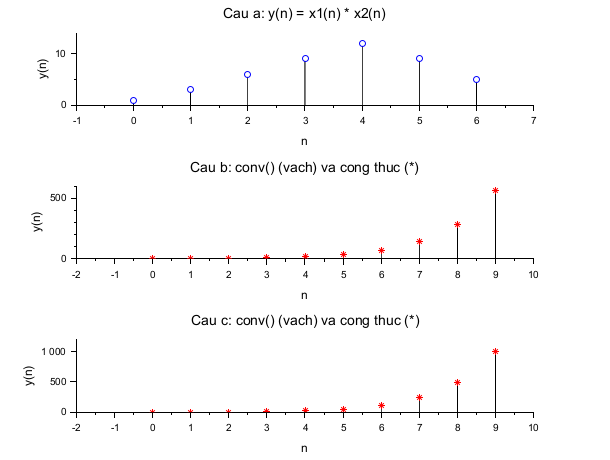
\includegraphics[width=0.8\linewidth]{img/Ex2_dothi.png}
    \caption{Exercise 2 -- kết quả \texttt{conv()} (vạch) và công thức tính tay (dấu *)}
\end{figure}
\begin{figure}[H]
    \centering
    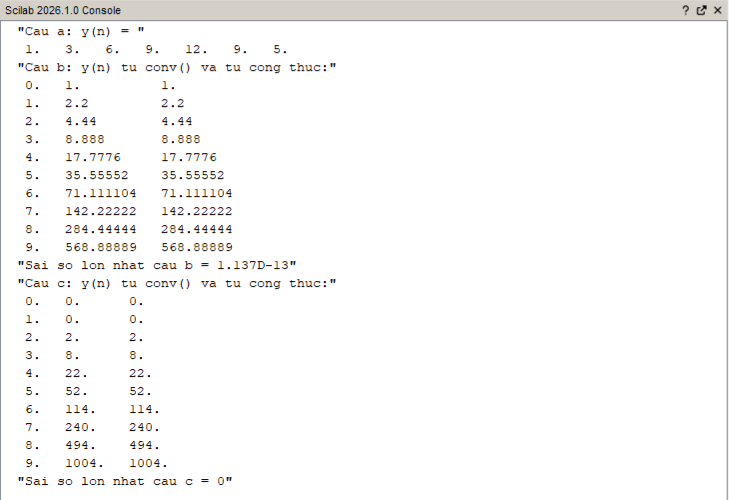
\includegraphics[width=0.75\linewidth]{img/Ex2_console_crop.png}
    \caption{Exercise 2 -- ảnh chụp cửa sổ Console: hai cột trùng nhau, sai số $\approx 10^{-13}$ (b) và $0$ (c)}
\end{figure}
\noindent\textbf{Nhận xét:} giá trị tính bằng \texttt{conv()} trùng với kết quả biến đổi $Z$ ngược ở cả ba câu; sai số ở câu (b) chỉ là sai số làm tròn số thực dấu phẩy động.

\subsection*{4.3 Exercise 3}
\textbf{Đề bài.} Tìm tất cả các $x(n)$ có biến đổi $Z$ cho dưới đây.

\par\smallskip\noindent\textbf{(1) $X_1(z)=\dfrac{1}{2-3z^{-1}+z^{-2}}$}\par
Đưa mẫu về dạng chuẩn: $X_1(z)=\dfrac{1/2}{1-\frac32z^{-1}+\frac12z^{-2}}=\dfrac{1/2}{(1-z^{-1})(1-\frac12z^{-1})}$, cực tại $z=1$ và $z=0{,}5$.
\[
A=\left.\frac{1/2}{1-\frac12z^{-1}}\right|_{z^{-1}=1}=1,\qquad
B=\left.\frac{1/2}{1-z^{-1}}\right|_{z^{-1}=2}=-\frac12,
\]
\[
X_1(z)=\frac{1}{1-z^{-1}}-\frac{1/2}{1-0{,}5z^{-1}}.
\]
Hai cực chia mặt phẳng $z$ thành ba ROC, ứng với ba tín hiệu:
\begin{itemize}[leftmargin=*]
    \item ROC $|z|>1$ (nhân quả): $x_1(n)=\left[1-(0{,}5)^{n+1}\right]u(n)$.
    \item ROC $0{,}5<|z|<1$ (hai phía): $x_1(n)=-u(-n-1)-(0{,}5)^{n+1}u(n)$.
    \item ROC $|z|<0{,}5$ (phản nhân quả): $x_1(n)=\left[-1+(0{,}5)^{n+1}\right]u(-n-1)$.
\end{itemize}

\par\smallskip\noindent\textbf{(2) $X_2(z)=\dfrac{1+2z^{-1}+z^{-2}}{1+4z^{-1}+4z^{-2}}$}\par
$X_2(z)=\left(\dfrac{1+z^{-1}}{1+2z^{-1}}\right)^2$ có cực kép tại $z=-2$. Vì $\dfrac{1+z^{-1}}{1+2z^{-1}}=\dfrac12+\dfrac{1/2}{1+2z^{-1}}$ nên
\[
X_2(z)=\frac14+\frac{1/2}{1+2z^{-1}}+\frac{1/4}{(1+2z^{-1})^2}.
\]
Dùng thêm cặp $-(n+1)a^nu(-n-1)\leftrightarrow\dfrac{1}{(1-az^{-1})^2}$, $|z|<|a|$, ta có hai trường hợp:
\begin{itemize}[leftmargin=*]
    \item ROC $|z|>2$ (nhân quả): $x_2(n)=\tfrac14\delta(n)+\tfrac{n+3}{4}(-2)^nu(n)$.
    \item ROC $|z|<2$ (phản nhân quả): $x_2(n)=\tfrac14\delta(n)-\tfrac{n+3}{4}(-2)^nu(-n-1)$.
\end{itemize}

\par\smallskip\noindent\textbf{(3) $X_3(z)=\dfrac{1+z^{-1}}{(1-0{,}5z^{-1})^2(1-0{,}3z^{-1})}$, ROC $0{,}3<|z|<0{,}5$}\par
(Đề ghi $0{,}3<z<0{,}5$, hiểu là $0{,}3<|z|<0{,}5$.) Khai triển
\[
X_3(z)=\frac{A}{1-0{,}3z^{-1}}+\frac{B}{1-0{,}5z^{-1}}+\frac{C}{(1-0{,}5z^{-1})^2}.
\]
\begin{itemize}[leftmargin=*]
    \item $A=\left.\dfrac{1+z^{-1}}{(1-0{,}5z^{-1})^2}\right|_{z^{-1}=10/3}=\dfrac{13/3}{4/9}=\dfrac{39}{4}$.
    \item $C=\left.\dfrac{1+z^{-1}}{1-0{,}3z^{-1}}\right|_{z^{-1}=2}=\dfrac{3}{0{,}4}=\dfrac{15}{2}$.
    \item Cho $z^{-1}=0$: $1=A+B+C\Rightarrow B=-\dfrac{65}{4}$.
\end{itemize}
Với ROC $0{,}3<|z|<0{,}5$: cực $z=0{,}3$ nằm trong (cho thành phần nhân quả), cực kép $z=0{,}5$ nằm ngoài (cho thành phần phản nhân quả):
\[
x_3(n)=\frac{39}{4}(0{,}3)^nu(n)+\frac{65}{4}(0{,}5)^nu(-n-1)-\frac{15}{2}(n+1)(0{,}5)^nu(-n-1)
\]
\[
\boxed{\,x_3(n)=\frac{39}{4}(0{,}3)^nu(n)+\frac{35-30n}{4}(0{,}5)^nu(-n-1)\,}
\]

\subsection*{4.4 Exercise 4}
\textbf{Đề bài.} Cho hệ LTI mô tả bởi phương trình $y(n) = 0{,}7\,y(n-1) + x(n)$.
(a) Vẽ sơ đồ khối; (b) xác định $h(n)$; (c) xác định $y(n)$ khi $x(n) = u(n)$.

\par\smallskip\noindent\textbf{(a) Sơ đồ khối}\par
Ngõ ra $y(n)$ được làm trễ một mẫu (khối $z^{-1}$), nhân hệ số $0{,}7$ rồi cộng với ngõ vào $x(n)$:
\begin{figure}[H]
\centering
\begin{tikzpicture}[>=Stealth, thick]
    \node (x) at (0,0) {$x(n)$};
    \node[draw, circle, minimum size=7mm, inner sep=0pt] (s) at (2.4,0) {$+$};
    \coordinate (t) at (5.4,0);
    \node (y) at (7.6,0) {$y(n)$};
    \node[draw, minimum width=12mm, minimum height=8mm] (d) at (5.4,-1.9) {$z^{-1}$};
    \node[draw, isosceles triangle, shape border rotate=180, minimum height=10mm, minimum width=9mm, inner sep=1pt] (g) at (3.6,-1.9) {};
    \node[above=2pt] at (g.north) {$0{,}7$};
    \draw[->] (x) -- (s);
    \draw[->] (s) -- (y);
    \fill (t) circle (2pt);
    \draw[->] (t) -- (d);
    \draw[->] (d) -- (g.east);
    \draw[->] (g.apex) -| (s.south);
    \node[right] at (5.4,-1.0) {$y(n-1)$};
\end{tikzpicture}
\caption{Sơ đồ khối của hệ $y(n) = 0{,}7\,y(n-1) + x(n)$}
\end{figure}

\par\smallskip\noindent\textbf{(b) Đáp ứng xung $h(n)$}\par
Lấy biến đổi $Z$ hai vế (hệ LTI nhân quả, điều kiện đầu bằng 0), dùng tính chất dịch $y(n-1)\leftrightarrow z^{-1}Y(z)$:
\[
Y(z) = 0{,}7\,z^{-1}Y(z) + X(z) \;\Rightarrow\; H(z) = \frac{Y(z)}{X(z)} = \frac{1}{1-0{,}7z^{-1}}, \qquad \text{ROC: } |z| > 0{,}7.
\]
Hệ nhân quả nên ROC là miền ngoài cực $p = 0{,}7$. Lấy $Z^{-1}$:
\[
\boxed{\,h(n) = (0{,}7)^n u(n)\,}
\]
Cực $p=0{,}7$ nằm trong vòng tròn đơn vị nên hệ ổn định (ROC chứa $|z|=1$).

\par\smallskip\noindent\textbf{(c) Đáp ứng khi $x(n) = u(n)$}\par
$X(z) = \dfrac{1}{1-z^{-1}}$, $|z|>1$, nên
\[
Y(z) = H(z)X(z) = \frac{1}{(1-0{,}7z^{-1})(1-z^{-1})} = \frac{A}{1-0{,}7z^{-1}} + \frac{B}{1-z^{-1}}, \qquad |z| > 1,
\]
\[
A = \left.\frac{1}{1-z^{-1}}\right|_{z^{-1}=\frac{1}{0{,}7}} = \frac{1}{1-\frac{10}{7}} = -\frac{7}{3}, \qquad
B = \left.\frac{1}{1-0{,}7z^{-1}}\right|_{z^{-1}=1} = \frac{1}{0{,}3} = \frac{10}{3}.
\]
\[
\boxed{\,y(n) = \left[\frac{10}{3} - \frac{7}{3}(0{,}7)^n\right]u(n)\,}
\]
Kiểm tra bằng phương trình sai phân: $y(0) = 1$, $y(1) = 0{,}7\cdot 1 + 1 = 1{,}7$, $y(2) = 0{,}7\cdot1{,}7+1 = 2{,}19$; công thức cho $y(1) = \frac{10}{3} - \frac{7}{3}\cdot 0{,}7 = 1{,}7$. \checkmark
Khi $n\to\infty$, $y(n)\to \frac{10}{3} \approx 3{,}333 = H(1)$ (độ lợi DC của hệ).
\Needspace{12\baselineskip}\par\smallskip\noindent\textbf{Mô phỏng bằng Scilab}\par
Dùng \texttt{filter(b, a, x)} với $b = 1$, $a = [1\;\; -0{,}7]$ để mô phỏng hệ theo phương trình sai phân, với ngõ vào là xung đơn vị $\delta(n)$ (câu b) và bước đơn vị $u(n)$ (câu c).
\begin{figure}[H]
    \centering
    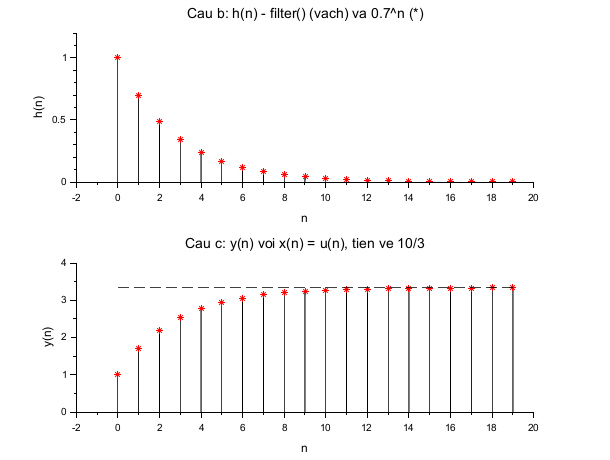
\includegraphics[width=0.8\linewidth]{img/Ex4_dothi.png}
    \caption{Exercise 4 -- $h(n)$ và $y(n)$ mô phỏng (vạch) so với công thức (dấu *); đường nét đứt là giá trị xác lập $10/3$}
\end{figure}
\begin{figure}[H]
    \centering
    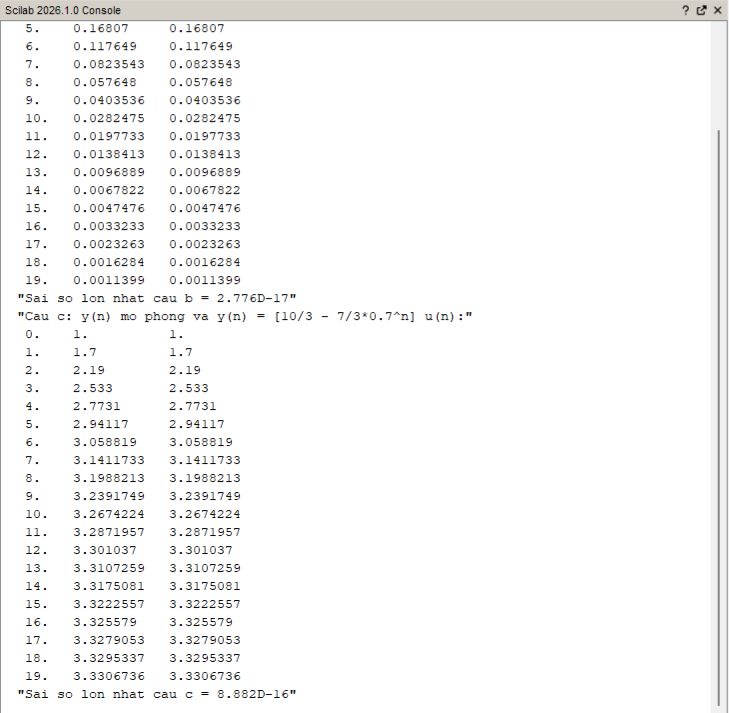
\includegraphics[width=0.7\linewidth]{img/Ex4_console_crop.png}
    \caption{Exercise 4 -- ảnh chụp Console: cột mô phỏng và cột công thức của câu (c) trùng nhau, sai số $\approx 10^{-16}$}
\end{figure}

\subsection*{4.5 Exercise 5}
\textbf{Đề bài.} Cho hệ LTI $y(n)=2y(n-1)-3y(n-2)+x(n)+x(n-1)$. (a) Vẽ sơ đồ khối; (b) tìm $h(n)$; (c) tìm $y_{zi}(n)$ khi $y(-1)=y(-2)=1$; (d) tìm $y_{zs}(n)$ khi $x(n)=2^nu(n)$.

\par\smallskip\noindent\textbf{(a) Sơ đồ khối (Direct Form I)}\par
Phần tử số (bên trái) tạo $x(n)+x(n-1)$; phần hồi tiếp (bên phải) cộng thêm $2y(n-1)$ và $-3y(n-2)$. Hệ không có số hạng $x(n-2)$ nên nhánh tử số chỉ cần một khối trễ.
\begin{figure}[H]
\centering
\begin{tikzpicture}[>=Stealth, thick,
    sum/.style={draw, circle, minimum size=7mm, inner sep=0pt},
    del/.style={draw, minimum width=11mm, minimum height=8mm},
    gain/.style={draw, isosceles triangle, minimum height=9mm, minimum width=8mm, inner sep=1pt}]
    \node (x) at (0,0) {$x(n)$};
    \coordinate (xs) at (1.3,0);
    \node[gain] (b0) at (2.6,0) {};
    \node[above=2pt] at (b0.north) {$1$};
    \node[sum] (s1) at (4.2,0) {$+$};
    \node[del] (dx) at (1.3,-1.6) {$z^{-1}$};
    \node[gain] (b1) at (2.6,-3.0) {};
    \node[above=2pt] at (b1.north) {$1$};
    \node[sum] (s2) at (5.6,0) {$+$};
    \coordinate (ys) at (8.6,0);
    \node (y) at (10.2,0) {$y(n)$};
    \node[del] (dy1) at (8.6,-1.5) {$z^{-1}$};
    \node[del] (dy2) at (8.6,-3.4) {$z^{-1}$};
    \node[gain, shape border rotate=180] (a1) at (7.1,-2.35) {};
    \node[above=2pt] at (a1.north) {$2$};
    \node[gain, shape border rotate=180] (a2) at (7.1,-4.25) {};
    \node[above=2pt] at (a2.north) {$-3$};
    \node[sum] (s3) at (5.6,-2.35) {$+$};
    \draw[->] (x) -- (b0.west);
    \fill (xs) circle (2pt);
    \draw[->] (b0.east) -- (s1);
    \draw[->] (xs) -- (dx);
    \draw (dx.south) -- (1.3,-3.0);
    \draw[->] (1.3,-3.0) -- (b1.west);
    \node[left] at (1.3,-3.0) {$x(n-1)$};
    \draw[->] (b1.east) -| (s1.south);
    \draw[->] (s1) -- (s2);
    \draw[->] (s2) -- (y);
    \fill (ys) circle (2pt);
    \draw[->] (ys) -- (dy1);
    \draw[->] (dy1) -- (dy2);
    \coordinate (y1) at (8.6,-2.35);
    \fill (y1) circle (2pt);
    \draw[->] (y1) -- (a1.west);
    \node[right] at (8.6,-2.35) {$y(n-1)$};
    \draw (dy2.south) -- (8.6,-4.25);
    \draw[->] (8.6,-4.25) -- (a2.west);
    \node[right] at (8.6,-4.25) {$y(n-2)$};
    \draw[->] (a1.east) -- (s3);
    \draw[->] (a2.east) -| (s3.south);
    \draw[->] (s3) -- (s2);
\end{tikzpicture}
\caption{Sơ đồ khối Direct Form I của hệ $y(n)=2y(n-1)-3y(n-2)+x(n)+x(n-1)$}
\end{figure}

\par\smallskip\noindent\textbf{(b) Đáp ứng xung $h(n)$}\par
Lấy biến đổi $Z$ với điều kiện đầu bằng 0:
\[
Y(z)\left(1-2z^{-1}+3z^{-2}\right)=X(z)\left(1+z^{-1}\right)\;\Rightarrow\;
H(z)=\frac{1+z^{-1}}{1-2z^{-1}+3z^{-2}}.
\]
Cực là nghiệm của $z^2-2z+3=0$: $z=1\pm j\sqrt2=\sqrt3\,e^{\pm j\theta}$ với $r=\sqrt3$, $\cos\theta=\tfrac{1}{\sqrt3}$, $\sin\theta=\sqrt{\tfrac23}$, tức $\theta=\arctan\sqrt2\approx0{,}9553$ rad. Khi đó $r\cos\theta=1$, $r\sin\theta=\sqrt2$, nên mẫu số có dạng chuẩn $1-2r\cos\theta\,z^{-1}+r^2z^{-2}$. Tách tử số $1+z^{-1}=(1-z^{-1})+\sqrt2\cdot\sqrt2\,z^{-1}$:
\[
H(z)=\frac{1-z^{-1}}{1-2z^{-1}+3z^{-2}}+\sqrt2\,\frac{\sqrt2\,z^{-1}}{1-2z^{-1}+3z^{-2}}
\]
\[
\boxed{\,h(n)=\left(\sqrt3\right)^n\left[\cos(n\theta)+\sqrt2\sin(n\theta)\right]u(n)\,}
\]
Kiểm tra: $h(0)=1$, $h(1)=\sqrt3\left(\tfrac{1}{\sqrt3}+\sqrt2\sqrt{\tfrac23}\right)=3$, trùng với $h(1)=2h(0)+1$ từ phương trình sai phân. Vì $r=\sqrt3>1$, hệ không ổn định.

\par\smallskip\noindent\textbf{(c) Đáp ứng không vào $y_{zi}(n)$ với $y(-1)=y(-2)=1$}\par
Cho $x(n)=0$, dùng biến đổi $Z$ một phía:
$Z^{+}\{y(n-1)\}=z^{-1}Y^{+}(z)+y(-1)$, $\;Z^{+}\{y(n-2)\}=z^{-2}Y^{+}(z)+z^{-1}y(-1)+y(-2)$.
\[
Y_{zi}(z)-2\left[z^{-1}Y_{zi}(z)+1\right]+3\left[z^{-2}Y_{zi}(z)+z^{-1}+1\right]=0
\;\Rightarrow\;
Y_{zi}(z)=\frac{-1-3z^{-1}}{1-2z^{-1}+3z^{-2}}.
\]
Tách $-1-3z^{-1}=-(1-z^{-1})-2\sqrt2\cdot\sqrt2\,z^{-1}$:
\[
Y_{zi}(z)=-\frac{1-z^{-1}}{1-2z^{-1}+3z^{-2}}-2\sqrt2\,\frac{\sqrt2\,z^{-1}}{1-2z^{-1}+3z^{-2}}
\]
\[
\boxed{\,y_{zi}(n)=-\left(\sqrt3\right)^n\left[\cos(n\theta)+2\sqrt2\sin(n\theta)\right]u(n)\,}
\]
Kiểm tra: từ phương trình sai phân $y(0)=2y(-1)-3y(-2)=-1$ và $y(1)=2y(0)-3y(-1)=-5$; công thức cho $y_{zi}(0)=-1$, $y_{zi}(1)=-\sqrt3\left(\tfrac{1}{\sqrt3}+2\sqrt2\sqrt{\tfrac23}\right)=-5$.

\par\smallskip\noindent\textbf{(d) Đáp ứng trạng thái không $y_{zs}(n)$ với $x(n)=2^nu(n)$}\par
$X(z)=\dfrac{1}{1-2z^{-1}}$, $|z|>2$, điều kiện đầu bằng 0:
\[
Y_{zs}(z)=H(z)X(z)=\frac{1+z^{-1}}{(1-2z^{-1})(1-2z^{-1}+3z^{-2})}=\frac{A}{1-2z^{-1}}+\frac{B+Cz^{-1}}{1-2z^{-1}+3z^{-2}}.
\]
$A=\left.\dfrac{1+z^{-1}}{1-2z^{-1}+3z^{-2}}\right|_{z^{-1}=1/2}=\dfrac{3/2}{3/4}=2$. Phần còn lại: $(1+z^{-1})-2(1-2z^{-1}+3z^{-2})=(1-2z^{-1})(-1+3z^{-1})$, nên $B+Cz^{-1}=-1+3z^{-1}=-(1-z^{-1})+\sqrt2\cdot\sqrt2\,z^{-1}$:
\[
\boxed{\,y_{zs}(n)=\left[2^{n+1}-\left(\sqrt3\right)^n\cos(n\theta)+\sqrt2\left(\sqrt3\right)^n\sin(n\theta)\right]u(n)\,}
\]
Kiểm tra: $y_{zs}(0)=2-1=1=x(0)$, $y_{zs}(1)=4+(-1+2)=5=2\cdot1+x(1)+x(0)$, đúng. (Trong tất cả các biểu thức, $\theta=\arctan\sqrt2$.)

\subsection*{4.6 Exercise 6}
\textbf{Đề bài.} Cho $x(n)\xleftrightarrow{Z} X(z)$ với ROC: $r_2 < |z| < r_1$. Chứng minh các tính chất sau.

\noindent Trong các chứng minh dưới đây ta dùng hai nhận xét: liên hợp phức có thể đưa vào trong tổng, và $\left(z^{-n}\right)^* = (z^*)^{-n}$. Ngoài ra ROC của biến đổi $Z$ chỉ phụ thuộc vào $|z|$, mà $|z^*| = |z|$ và $|ze^{-j\omega_0}| = |z|$.

\par\smallskip\noindent\textbf{(1) $Z\{x^*(n)\} = X^*(z^*)$}\par
\begin{align*}
Z\{x^*(n)\} &= \sum_{n=-\infty}^{\infty} x^*(n)\,z^{-n}
 = \sum_{n=-\infty}^{\infty} \left[x(n)\,(z^*)^{-n}\right]^*
 = \left[\sum_{n=-\infty}^{\infty} x(n)\,(z^*)^{-n}\right]^*
 = X^*(z^*).
\end{align*}
Chuỗi hội tụ khi $z^*$ thuộc ROC của $X$, tức $r_2 < |z^*| = |z| < r_1$: ROC không đổi. \hfill$\blacksquare$

\par\smallskip\noindent\textbf{(2) $Z\{\operatorname{Re}[x(n)]\} = \frac{1}{2}\left[X(z) + X^*(z^*)\right]$}\par
Ta có $\operatorname{Re}[x(n)] = \frac{1}{2}\left[x(n) + x^*(n)\right]$. Dùng tính chất tuyến tính và kết quả (1):
\[
Z\{\operatorname{Re}[x(n)]\} = \frac{1}{2}Z\{x(n)\} + \frac{1}{2}Z\{x^*(n)\} = \frac{1}{2}\left[X(z) + X^*(z^*)\right],
\]
ROC chứa ROC của $X(z)$. \hfill$\blacksquare$

\par\smallskip\noindent\textbf{(3) $Z\{\operatorname{Im}[x(n)]\} = \frac{1}{2j}\left[X(z) - X^*(z^*)\right]$}\par
Ta có $\operatorname{Im}[x(n)] = \frac{1}{2j}\left[x(n) - x^*(n)\right]$. Tương tự:
\[
Z\{\operatorname{Im}[x(n)]\} = \frac{1}{2j}Z\{x(n)\} - \frac{1}{2j}Z\{x^*(n)\} = \frac{1}{2j}\left[X(z) - X^*(z^*)\right],
\]
ROC chứa ROC của $X(z)$. \hfill$\blacksquare$

\par\smallskip\noindent\textbf{(4) $Z\{e^{j\omega_0 n}x(n)\} = X(z e^{-j\omega_0})$}\par
\[
Z\{e^{j\omega_0 n}x(n)\} = \sum_{n=-\infty}^{\infty} x(n)\,e^{j\omega_0 n} z^{-n}
 = \sum_{n=-\infty}^{\infty} x(n)\left(z e^{-j\omega_0}\right)^{-n} = X(z e^{-j\omega_0}).
\]
Chuỗi hội tụ khi $r_2 < |ze^{-j\omega_0}| = |z| < r_1$ nên ROC không đổi. Về ý nghĩa, nhân với $e^{j\omega_0 n}$ làm toàn bộ giản đồ cực -- không quay một góc $\omega_0$ quanh gốc tọa độ (dịch tần số $\omega_0$ trên phổ). \hfill$\blacksquare$
\Needspace{12\baselineskip}\par\smallskip\noindent\textbf{Kiểm chứng bằng Scilab}\par
Bài này là bài chứng minh nên không cần mô phỏng đồ thị; tuy vậy có thể kiểm tra số học cả 4 đẳng thức. Chọn một tín hiệu phức hữu hạn $x(n) = \{\underset{\uparrow}{1+2j},\, 3-j,\, -2j,\, 4,\, 1+j\}$, một điểm bất kỳ $z_0 = 1{,}5e^{j\pi/5}$ và $\omega_0 = \pi/3$, rồi tính vế trái (VT) và vế phải (VP) của từng đẳng thức theo định nghĩa $X(z)=\sum x(n)z^{-n}$.
\begin{table}[H]
    \centering
    \begin{tabular}{|c|c|c|c|}
        \hline
        Tính chất & VT & VP & $|\text{VT}-\text{VP}|$ \\
        \hline
        (1) & $3{,}2131 - 3{,}4450j$ & $3{,}2131 - 3{,}4450j$ & $0$ \\
        (2) & $2{,}0920 - 2{,}4189j$ & $2{,}0920 - 2{,}4189j$ & $4{,}4\cdot10^{-16}$ \\
        (3) & $1{,}0262 + 1{,}1211j$ & $1{,}0262 + 1{,}1211j$ & $2{,}2\cdot10^{-16}$ \\
        (4) & $3{,}9080 + 2{,}9126j$ & $3{,}9080 + 2{,}9126j$ & $1{,}4\cdot10^{-15}$ \\
        \hline
    \end{tabular}
    \caption{Exercise 6 -- so sánh hai vế tại $z_0 = 1{,}5e^{j\pi/5}$}
\end{table}
\begin{figure}[H]
    \centering
    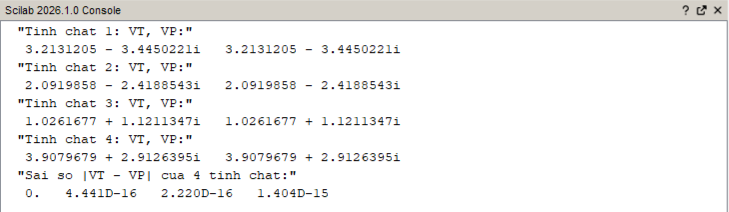
\includegraphics[width=0.75\linewidth]{img/Ex6_console_crop.png}
    \caption{Exercise 6 -- ảnh chụp Console}
\end{figure}

\subsection*{4.7 Bài tập thêm (Additional Exercises)}

\subsubsection*{Bài 3.3}
\textbf{Đề bài.} Tìm biến đổi $Z$ và phác họa ROC của các tín hiệu:
$x_1(n)=\left(\tfrac13\right)^n$ khi $n\ge0$, $\left(\tfrac12\right)^{-n}$ khi $n<0$; $\;x_2(n)=\left(\tfrac13\right)^n-2^n$ khi $n\ge0$, 0 khi $n<0$; $\;x_3(n)=x_1(n+4)$; $\;x_4(n)=x_1(-n)$.

\noindent\textbf{(a)} Với $n<0$, $\left(\tfrac12\right)^{-n}=2^n$, nên $x_1(n)=\left(\tfrac13\right)^nu(n)+2^nu(-n-1)$.
\begin{itemize}[leftmargin=*]
    \item $\left(\tfrac13\right)^nu(n)\leftrightarrow\dfrac{1}{1-\frac13z^{-1}}$, $|z|>\tfrac13$.
    \item $2^nu(-n-1)\leftrightarrow-\dfrac{1}{1-2z^{-1}}$, $|z|<2$.
\end{itemize}
\[
X_1(z)=\frac{1}{1-\frac13z^{-1}}-\frac{1}{1-2z^{-1}}=\frac{-\frac53z^{-1}}{\left(1-\frac13z^{-1}\right)\left(1-2z^{-1}\right)},\qquad \tfrac13<|z|<2.
\]

\noindent\textbf{(b)} $x_2(n)=\left[\left(\tfrac13\right)^n-2^n\right]u(n)$ là tín hiệu nhân quả:
\[
X_2(z)=\frac{1}{1-\frac13z^{-1}}-\frac{1}{1-2z^{-1}}=\frac{-\frac53z^{-1}}{\left(1-\frac13z^{-1}\right)\left(1-2z^{-1}\right)},\qquad |z|>2.
\]
$X_2(z)$ có cùng biểu thức với $X_1(z)$ nhưng khác ROC, cho thấy phải có ROC mới xác định được tín hiệu.

\noindent\textbf{(c)} $x_3(n)=x_1(n+4)$ (dịch trái 4 mẫu). Theo tính chất dịch thời gian $x(n+k)\leftrightarrow z^{k}X(z)$:
\[
X_3(z)=z^4X_1(z)=\frac{-\frac53z^{3}}{\left(1-\frac13z^{-1}\right)\left(1-2z^{-1}\right)},\qquad \tfrac13<|z|<2.
\]
Dịch thời gian không đổi vị trí cực nên ROC giữ nguyên như câu (a).

\noindent\textbf{(d)} $x_4(n)=x_1(-n)$. Theo tính chất đảo thời gian $x(-n)\leftrightarrow X(z^{-1})$, ROC nghịch đảo:
\[
X_4(z)=X_1\!\left(\tfrac1z\right)=\frac{1}{1-\frac13z}-\frac{1}{1-2z}=\frac{-3z^{-1}}{1-3z^{-1}}+\frac{0{,}5z^{-1}}{1-0{,}5z^{-1}}=\frac{-2{,}5z^{-1}}{1-3{,}5z^{-1}+1{,}5z^{-2}},
\]
với ROC $\tfrac13<\tfrac{1}{|z|}<2$, tức $0{,}5<|z|<3$.

\begin{figure}[H]
\centering
\newcommand{\rocplot}[4]{%
\begin{tikzpicture}[scale=0.55]
  #1
  \draw[->] (-3.4,0) -- (3.6,0) node[right] {\scriptsize Re};
  \draw[->] (0,-3.4) -- (0,3.6) node[above] {\scriptsize Im};
  #2
  \node at (0,-4.1) {\small #3};
  #4
\end{tikzpicture}}
\rocplot{\fill[green!35] (0,0) circle (2); \fill[white] (0,0) circle (0.333);}
  {\draw[dashed] (0,0) circle (2); \draw[dashed] (0,0) circle (0.333);
   \node at (0.333,0) {$\times$}; \node at (2,0) {$\times$};
   \node[below right] at (2,0) {\scriptsize 2};}
  {(a), (c): $\tfrac13<|z|<2$}{}
\hspace{0.5cm}
\rocplot{\fill[green!35] (-3.3,-3.3) rectangle (3.3,3.3); \fill[white] (0,0) circle (2);}
  {\draw[dashed] (0,0) circle (2);
   \node at (0.333,0) {$\times$}; \node at (2,0) {$\times$};
   \node[below right] at (2,0) {\scriptsize 2};}
  {(b): $|z|>2$}{}
\hspace{0.5cm}
\rocplot{\fill[green!35] (0,0) circle (3); \fill[white] (0,0) circle (0.5);}
  {\draw[dashed] (0,0) circle (3); \draw[dashed] (0,0) circle (0.5);
   \node at (0.5,0) {$\times$}; \node at (3,0) {$\times$};
   \node[below right] at (3,0) {\scriptsize 3};}
  {(d): $0{,}5<|z|<3$}{}
\caption{Bài 3.3 -- ROC (vùng tô màu) và vị trí các cực ($\times$)}
\end{figure}

\subsubsection*{Bài 3.4}
\textbf{Đề bài.} Xác định biến đổi $Z$ của các tín hiệu:
(a) $n(-1)^n u(n)$; (b) $n^2 u(n)$; (c) $-n a^n u(-n-1)$; (d) $(-1)^n\cos\left(\frac{\pi}{3}n\right)u(n)$; (e) $(-1)^n u(n)$; (f) $x(n) = \{\underset{\uparrow}{1}, 0, -1, 0, 1, -1, \dots\}$.

\noindent\textbf{Các cặp và tính chất sử dụng:}
\begin{gather*}
a^n u(n) \leftrightarrow \frac{1}{1-az^{-1}} = \frac{z}{z-a},\ |z|>|a|; \qquad
-a^n u(-n-1) \leftrightarrow \frac{1}{1-az^{-1}},\ |z|<|a|; \\
n\,x(n) \leftrightarrow -z\frac{dX(z)}{dz} \quad \text{(đạo hàm trong miền } z\text{)}.
\end{gather*}

\par\smallskip\noindent\textbf{(e) $x(n) = (-1)^n u(n)$}\par
Làm câu (e) trước vì được dùng cho câu (a). Với $a = -1$:
\[
\boxed{\,X(z) = \frac{1}{1+z^{-1}} = \frac{z}{z+1}, \qquad |z| > 1\,}
\]

\par\smallskip\noindent\textbf{(a) $x(n) = n(-1)^n u(n)$}\par
Đặt $X_e(z) = \dfrac{z}{z+1}$ (câu e). Ta có $\dfrac{dX_e}{dz} = \dfrac{(z+1) - z}{(z+1)^2} = \dfrac{1}{(z+1)^2}$, nên
\[
\boxed{\,X(z) = -z\frac{dX_e(z)}{dz} = -\frac{z}{(z+1)^2} = -\frac{z^{-1}}{(1+z^{-1})^2}, \qquad |z| > 1\,}
\]

\par\smallskip\noindent\textbf{(b) $x(n) = n^2 u(n)$}\par
Từ $u(n)\leftrightarrow \frac{z}{z-1}$: $\;n\,u(n) \leftrightarrow -z\frac{d}{dz}\left(\frac{z}{z-1}\right) = -z\cdot\frac{-1}{(z-1)^2} = \frac{z}{(z-1)^2}$. Áp dụng thêm một lần nữa:
\[
n^2u(n) \leftrightarrow -z\frac{d}{dz}\left[\frac{z}{(z-1)^2}\right]
 = -z\cdot\frac{(z-1)^2 - 2z(z-1)}{(z-1)^4}
 = -z\cdot\frac{(z-1)-2z}{(z-1)^3} = \frac{z(z+1)}{(z-1)^3}.
\]
\[
\boxed{\,X(z) = \frac{z(z+1)}{(z-1)^3} = \frac{z^{-1}(1+z^{-1})}{(1-z^{-1})^3}, \qquad |z| > 1\,}
\]

\par\smallskip\noindent\textbf{(c) $x(n) = -n a^n u(-n-1)$}\par
Viết $x(n) = n\cdot\left[-a^nu(-n-1)\right]$ với $-a^nu(-n-1)\leftrightarrow \dfrac{z}{z-a}$, $|z|<|a|$ (tín hiệu phản nhân quả):
\[
X(z) = -z\frac{d}{dz}\left(\frac{z}{z-a}\right) = -z\cdot\frac{(z-a)-z}{(z-a)^2} = \frac{az}{(z-a)^2}.
\]
\[
\boxed{\,X(z) = \frac{az^{-1}}{(1-az^{-1})^2}, \qquad |z| < |a|\,}
\]

\par\smallskip\noindent\textbf{(d) $x(n) = (-1)^n\cos\left(\frac{\pi}{3}n\right)u(n)$}\par
Cặp cơ bản: $\cos(\omega_0 n)u(n) \leftrightarrow \dfrac{1 - z^{-1}\cos\omega_0}{1 - 2z^{-1}\cos\omega_0 + z^{-2}}$, $|z|>1$.
Tính chất co giãn miền $z$: $a^n x(n) \leftrightarrow X(a^{-1}z)$; với $a=-1$ tức là thay $z^{-1}$ bằng $-z^{-1}$:
\[
X(z) = \frac{1 + z^{-1}\cos\omega_0}{1 + 2z^{-1}\cos\omega_0 + z^{-2}}\Bigg|_{\omega_0 = \pi/3,\ \cos\omega_0 = 1/2}
\]
\[
\boxed{\,X(z) = \frac{1 + \frac{1}{2}z^{-1}}{1 + z^{-1} + z^{-2}}, \qquad |z| > 1\,}
\]
\textit{Kiểm tra cách khác:} $(-1)^n\cos\frac{\pi n}{3} = \frac{1}{2}\left(e^{j4\pi n/3} + e^{j2\pi n/3}\right) = \cos\frac{2\pi n}{3}$ (vì $e^{j4\pi n/3} = e^{-j2\pi n/3}$), và $\cos\frac{2\pi}{3} = -\frac12$ cho cùng kết quả trên.

\par\smallskip\noindent\textbf{(f) $x(n) = \{\underset{\uparrow}{1}, 0, -1, 0, 1, -1, \dots\}$}\par
Dãy trong đề là dãy nhân quả lặp lại theo mẫu $1, 0, -1, 0$ (giống lời giải tham khảo của sách, coi số hạng thứ 6 là lỗi in), tức $x(n) = \{\underset{\uparrow}{1}, 0, -1, 0, 1, 0, -1, 0, \dots\} = \cos\left(\frac{\pi}{2}n\right)u(n)$. Khi đó:
\[
X(z) = 1 - z^{-2} + z^{-4} - z^{-6} + \cdots = \sum_{k=0}^{\infty}\left(-z^{-2}\right)^k
\]
là cấp số nhân công bội $-z^{-2}$, hội tụ khi $|z^{-2}|<1$:
\[
\boxed{\,X(z) = \frac{1}{1+z^{-2}} = \frac{z^2}{z^2+1}, \qquad |z| > 1\,}
\]
(trùng với công thức $\cos(\omega_0 n)u(n)$ ở câu (d) với $\omega_0 = \pi/2$).
\textit{Ghi chú:} nếu hiểu đúng nguyên văn là dãy tuần hoàn chu kỳ 6 $\{1, 0, -1, 0, 1, -1\}$ thì $X(z) = \dfrac{1 - z^{-2} + z^{-4} - z^{-5}}{1 - z^{-6}}$, $|z|>1$.
\Needspace{12\baselineskip}\par\smallskip\noindent\textbf{Mô phỏng bằng Scilab}\par
Với mỗi tín hiệu, tính tổng riêng phần $\sum_{n} x(n)z_0^{-n}$ (300 mẫu) tại một điểm $z_0$ nằm trong ROC rồi so sánh với $X(z_0)$ tính từ công thức. Chọn $z_0 = 1{,}5$ (thỏa $|z|>1$); riêng câu (c) chọn $a = 2$ để $z_0 = 1{,}5$ thỏa $|z| < |a|$.
\begin{table}[H]
    \centering
    \begin{tabular}{|c|c|c|c|}
        \hline
        Câu & Tổng $\sum x(n) z_0^{-n}$ & Công thức $X(z_0)$ & Sai số \\
        \hline
        (a) & $-0{,}24$ & $-0{,}24$ & $1{,}7\cdot10^{-16}$ \\
        (b) & $30$ & $30$ & $7{,}1\cdot10^{-15}$ \\
        (c) & $12$ & $12$ & $5{,}3\cdot10^{-15}$ \\
        (d) & $0{,}63157895$ & $0{,}63157895$ & $1{,}1\cdot10^{-16}$ \\
        (e) & $0{,}6$ & $0{,}6$ & $2{,}2\cdot10^{-16}$ \\
        (f) & $0{,}69230769$ & $0{,}69230769$ & $1{,}1\cdot10^{-16}$ \\
        \hline
    \end{tabular}
    \caption{Bài 3.4 -- kiểm tra biến đổi $Z$ tại $z_0 = 1{,}5$}
\end{table}
\begin{figure}[H]
    \centering
    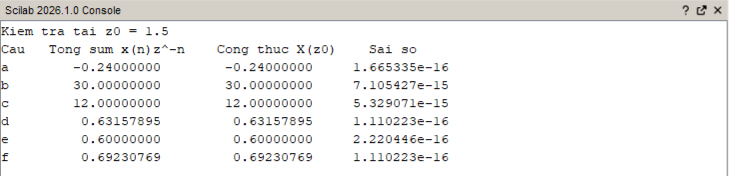
\includegraphics[width=0.75\linewidth]{img/BT3_4_console_crop.png}
    \caption{Bài 3.4 -- ảnh chụp Console}
\end{figure}
\begin{figure}[H]
    \centering
    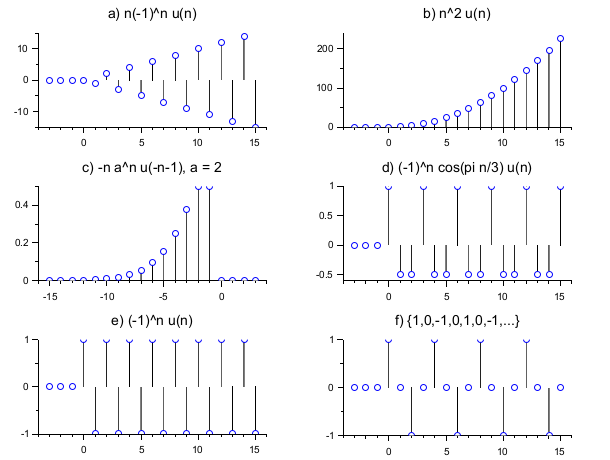
\includegraphics[width=0.85\linewidth]{img/BT3_4_dothi.png}
    \caption{Bài 3.4 -- dạng sóng các tín hiệu (vẽ thêm vài mẫu $n<0$ để thấy ảnh hưởng của $u(n)$, $u(-n-1)$)}
\end{figure}

\subsubsection*{Bài 3.7}
\textbf{Đề bài.} Tính tích chập $y(n)=x_1(n)*x_2(n)$ bằng biến đổi $Z$, với $x_1(n)$ như bài 3.3(a) và $x_2(n)=\left(\tfrac12\right)^nu(n)$.

Theo tính chất tích chập, $Y(z)=X_1(z)X_2(z)$. Từ bài 3.3(a):
\[
X_1(z)=\frac{-\frac53z^{-1}}{\left(1-\frac13z^{-1}\right)\left(1-2z^{-1}\right)},\ \ \tfrac13<|z|<2;\qquad
X_2(z)=\frac{1}{1-\frac12z^{-1}},\ \ |z|>\tfrac12.
\]
\[
Y(z)=\frac{-\frac53z^{-1}}{\left(1-\frac13z^{-1}\right)\left(1-\frac12z^{-1}\right)\left(1-2z^{-1}\right)},\qquad \tfrac12<|z|<2.
\]
Khai triển $Y(z)=\dfrac{A}{1-\frac13z^{-1}}+\dfrac{B}{1-\frac12z^{-1}}+\dfrac{C}{1-2z^{-1}}$:
\begin{itemize}[leftmargin=*]
    \item $z^{-1}=3$: $A\left(1-\tfrac32\right)(1-6)=-5\Rightarrow A=-2$.
    \item $z^{-1}=2$: $B\left(1-\tfrac23\right)(1-4)=-\tfrac{10}{3}\Rightarrow B=\tfrac{10}{3}$.
    \item $z^{-1}=\tfrac12$: $C\left(1-\tfrac16\right)\left(1-\tfrac14\right)=-\tfrac56\Rightarrow C=-\tfrac43$.
\end{itemize}
Với ROC $\tfrac12<|z|<2$: các cực $\tfrac13$, $\tfrac12$ nằm trong (thành phần nhân quả), cực $2$ nằm ngoài (thành phần phản nhân quả, dùng $-a^nu(-n-1)$):
\[
\boxed{\,y(n)=-2\left(\tfrac13\right)^nu(n)+\tfrac{10}{3}\left(\tfrac12\right)^nu(n)+\tfrac43\,2^nu(-n-1)\,}
\]

\subsubsection*{Bài 3.8}
\textbf{(a)} Vì \(u(n-k)=1\) khi và chỉ khi \(k\le n\), tổng tích lũy
viết được dưới dạng tích chập với \(u(n)\):

\[y(n)=\sum_{k=-\infty}^{n}x(k)=\sum_{k=-\infty}^{\infty}x(k)\,u(n-k)=x(n)*u(n).\]

Áp dụng tính chất tích chập với \(U(z)=\dfrac{1}{1-z^{-1}}\)
(\(|z|>1\)):

\[Y(z)=X(z)\,U(z)=\frac{X(z)}{1-z^{-1}},\qquad \text{ROC}_Y\supseteq\text{ROC}_X\cap\{|z|>1\}.\]

\textbf{(b)} Trước hết chứng minh \((n+1)u(n)=u(n)*u(n)\):

\[u(n)*u(n)=\sum_{k=-\infty}^{\infty}u(k)\,u(n-k).\]

Số hạng khác 0 khi \(k\ge0\) và \(k\le n\).

\begin{itemize}
\item
  Với \(n<0\): không có \(k\) nào thỏa cả hai điều kiện, tổng bằng 0.
\item
  Với \(n\ge0\): có đúng \(n+1\) giá trị \(k=0,1,\dots,n\), mỗi số hạng
  bằng 1, tổng bằng \(n+1\).
\end{itemize}

Vậy \(u(n)*u(n)=(n+1)u(n)=x(n)\). Theo tính chất tích chập:

\[X(z)=U(z)\cdot U(z)=\frac{1}{(1-z^{-1})^2}=\frac{z^2}{(z-1)^2},\qquad |z|>1.\]

\(X(z)\) có cực kép tại \(z=1\) và không kép tại \(z=0\).

\subsubsection*{Bài 3.13}
Giả sử \(X(z)\) có ROC \(r_1<|z|<r_2\).

\textbf{(a)} \(x_1(n)=x(n/2)\) khi \(n\) chẵn và bằng 0 khi \(n\) lẻ
(chèn một mẫu 0 giữa hai mẫu liên tiếp). Chỉ các \(n=2m\) đóng góp vào
tổng, với \(x_1(2m)=x(m)\):

\[X_1(z)=\sum_{n}x_1(n)z^{-n}=\sum_{m=-\infty}^{\infty}x(m)z^{-2m}=\sum_{m}x(m)\left(z^{2}\right)^{-m}=X(z^2).\]

Chuỗi hội tụ khi \(r_1<|z^2|<r_2\), tức ROC là
\(\sqrt{r_1}<|z|<\sqrt{r_2}\).

\textbf{(b)} \(x_2(n)=x(2n)\) (chỉ giữ các mẫu có chỉ số chẵn). Xét dãy
phụ

\[v(m)=\tfrac12\left[1+(-1)^m\right]x(m)=\begin{cases}x(m), & m \text{ chẵn}\\ 0, & m \text{ lẻ}\end{cases}\]

Vì \(\sum_m (-1)^m x(m)z^{-m}=\sum_m x(m)(-z)^{-m}=X(-z)\), ta có

\[V(z)=\tfrac12\left[X(z)+X(-z)\right].\]

Mặt khác, \(v(m)\) chỉ khác 0 tại \(m=2n\), nên
\(V(z)=\sum_n x(2n)z^{-2n}=X_2(z^2)\). Thay \(z\) bằng \(z^{1/2}\):

\[X_2(z)=\tfrac12\left[X\!\left(z^{1/2}\right)+X\!\left(-z^{1/2}\right)\right],\qquad r_1^2<|z|<r_2^2.\]

Biểu thức không phụ thuộc vào cách chọn nhánh căn bậc hai, vì đổi
\(z^{1/2}\) thành \(-z^{1/2}\) chỉ đổi chỗ hai số hạng.

\emph{Ví dụ:} với \(x(n)=0{,}5^n u(n)\), \(X(z)=\dfrac{1}{1-0{,}5z^{-1}}\):

\begin{itemize}
\item
  \(X_1(z)=\dfrac{1}{1-0{,}5z^{-2}}\), ứng với
  \(\{1,0,0{,}5,0,0{,}25,\dots\}\), đúng là \(x(n)\) đã chèn 0.
\item
  \(X_2(z)=\tfrac12\left[\dfrac{1}{1-0{,}5z^{-1/2}}+\dfrac{1}{1+0{,}5z^{-1/2}}\right]\) \(=\dfrac{1}{1-0{,}25z^{-1}}\),
  ứng với \(0{,}25^n u(n)=x(2n)\).
\end{itemize}

\subsubsection*{Bài 3.14}
Các tín hiệu đều nhân quả, nên ROC là miền ngoài đường tròn qua cực lớn
nhất và mọi số hạng đều nhân với \(u(n)\).

\textbf{(a)}
\(X(z)=\dfrac{1+3z^{-1}}{1+3z^{-1}+2z^{-2}}=\dfrac{1+3z^{-1}}{(1+z^{-1})(1+2z^{-1})}\),
cực tại \(z=-1\) và \(z=-2\).

Khai triển \(X(z)=\dfrac{A_1}{1+z^{-1}}+\dfrac{A_2}{1+2z^{-1}}\):

\[A_1=\left.\frac{1+3z^{-1}}{1+2z^{-1}}\right|_{z^{-1}=-1}=\frac{-2}{-1}=2,\qquad A_2=\left.\frac{1+3z^{-1}}{1+z^{-1}}\right|_{z^{-1}=-1/2}=\frac{-1/2}{1/2}=-1.\]

\[x(n)=\left[2(-1)^n-(-2)^n\right]u(n),\qquad |z|>2.\]

Kiểm tra: \(x(0)=2-1=1=X(\infty)\).

\textbf{(b)} \(X(z)=\dfrac{1}{1-z^{-1}+\frac12z^{-2}}\). Mẫu bằng 0 khi
\(z^2-z+\tfrac12=0\), nên cực
\(p_{1,2}=\tfrac12\pm\tfrac12j=\tfrac{1}{\sqrt2}e^{\pm j\pi/4}\).

So với dạng chuẩn \(1-2r\cos\omega_0 z^{-1}+r^2z^{-2}\):
\(r=\tfrac{1}{\sqrt2}\), \(\omega_0=\tfrac{\pi}{4}\), do đó
\(r\cos\omega_0=r\sin\omega_0=\tfrac12\). Tách tử số
\(1=\left(1-\tfrac12z^{-1}\right)+\tfrac12z^{-1}\):

\[X(z)=\frac{1-\frac12z^{-1}}{1-z^{-1}+\frac12z^{-2}}+\frac{\frac12z^{-1}}{1-z^{-1}+\frac12z^{-2}}\]

\[x(n)=\left(\tfrac{1}{\sqrt2}\right)^n\left[\cos\tfrac{\pi n}{4}+\sin\tfrac{\pi n}{4}\right]u(n)=\sqrt2\left(\tfrac{1}{\sqrt2}\right)^n\sin\tfrac{(n+1)\pi}{4}\,u(n),\qquad |z|>\tfrac{1}{\sqrt2}.\]

\textbf{(c)}
\(X(z)=\dfrac{z^{-6}+z^{-7}}{1-z^{-1}}=z^{-6}\dfrac{1}{1-z^{-1}}+z^{-7}\dfrac{1}{1-z^{-1}}\).

Vì \(\dfrac{1}{1-z^{-1}}\leftrightarrow u(n)\), theo tính chất dịch thời
gian:

\[x(n)=u(n-6)+u(n-7)=\begin{cases}0, & n<6\\ 1, & n=6\\ 2, & n\ge7\end{cases},\qquad |z|>1.\]

\textbf{(d)} \(X(z)=\dfrac{1+2z^{-2}}{1+z^{-2}}\). Bậc tử bằng bậc mẫu
nên chia trước:

\[X(z)=\frac{2(1+z^{-2})-1}{1+z^{-2}}=2-\frac{1}{1+z^{-2}}.\]

Mẫu \(1+z^{-2}\) ứng với \(r=1\), \(\omega_0=\tfrac{\pi}{2}\)
(\(\cos\omega_0=0\)), nên
\(\dfrac{1}{1+z^{-2}}\leftrightarrow\cos\tfrac{\pi n}{2}\,u(n)\):

\[x(n)=2\delta(n)-\cos\!\left(\tfrac{\pi n}{2}\right)u(n)=\{1\uparrow,0,1,0,-1,0,1,0,\dots\},\qquad |z|>1.\]

\textbf{(e)}
\(X(z)=\dfrac14\cdot\dfrac{1+6z^{-1}+z^{-2}}{(1-2z^{-1}+2z^{-2})(1-0{,}5z^{-1})}\).

Cực: \(z=0{,}5\) và
\(z^2-2z+2=0\Rightarrow z=1\pm j=\sqrt2e^{\pm j\pi/4}\). Khai triển

\[X(z)=\frac{A}{1-0{,}5z^{-1}}+\frac{B+Cz^{-1}}{1-2z^{-1}+2z^{-2}}.\]

\begin{itemize}
\item
  \(A=\left.\dfrac14\cdot\dfrac{1+6z^{-1}+z^{-2}}{1-2z^{-1}+2z^{-2}}\right|_{z^{-1}=2}=\dfrac14\cdot\dfrac{1+12+4}{1-4+8}=\dfrac{17}{20}=0{,}85\).
\item
  Quy đồng:
  \(\tfrac14(1+6z^{-1}+z^{-2})=A(1-2z^{-1}+2z^{-2})+(B+Cz^{-1})(1-0{,}5z^{-1})\).
\item
  Hệ số \(z^0\): \(0{,}25=A+B\Rightarrow B=-0{,}6\).
\item
  Hệ số \(z^{-2}\): \(0{,}25=2A-0{,}5C\Rightarrow C=2{,}9\).
\item
  Kiểm tra hệ số \(z^{-1}\): \(-2A+C-0{,}5B=-1{,}7+2{,}9+0{,}3=1{,}5\), đúng.
\end{itemize}

Với \(r=\sqrt2\), \(\omega_0=\tfrac{\pi}{4}\)
(\(r\cos\omega_0=r\sin\omega_0=1\)), viết lại
\(B+Cz^{-1}=-0{,}6\,(1-z^{-1})+2{,}3\,z^{-1}\):

\[x(n)=\left[0{,}85(0{,}5)^n+(\sqrt2)^n\left(-0{,}6\cos\tfrac{\pi n}{4}+2{,}3\sin\tfrac{\pi n}{4}\right)\right]u(n),\qquad |z|>\sqrt2.\]

Kiểm tra: \(x(0)=0{,}85-0{,}6=0{,}25=X(\infty)\). Cặp cực phức nằm ngoài đường
tròn đơn vị nên \(x(n)\) tăng không giới hạn: tín hiệu nhân quả nhưng hệ
tương ứng không ổn định.

\textbf{(f)}
\(X(z)=\dfrac{2-1{,}5z^{-1}}{1-1{,}5z^{-1}+0{,}5z^{-2}}=\dfrac{2-1{,}5z^{-1}}{(1-z^{-1})(1-0{,}5z^{-1})}\).

\[A_1=\left.\frac{2-1{,}5z^{-1}}{1-0{,}5z^{-1}}\right|_{z^{-1}=1}=\frac{0{,}5}{0{,}5}=1,\qquad A_2=\left.\frac{2-1{,}5z^{-1}}{1-z^{-1}}\right|_{z^{-1}=2}=\frac{-1}{-1}=1.\]

\[x(n)=\left[1+(0{,}5)^n\right]u(n),\qquad |z|>1.\]

\textbf{(g)}
\(X(z)=\dfrac{1+2z^{-1}+z^{-2}}{1+4z^{-1}+4z^{-2}}=\left(\dfrac{1+z^{-1}}{1+2z^{-1}}\right)^2\),
cực kép tại \(z=-2\).

Vì \(1+z^{-1}=\tfrac12(1+2z^{-1})+\tfrac12\), ta có
\(\dfrac{1+z^{-1}}{1+2z^{-1}}=\dfrac12+\dfrac{1/2}{1+2z^{-1}}\). Bình
phương lên:

\[X(z)=\frac14+\frac{1/2}{1+2z^{-1}}+\frac{1/4}{(1+2z^{-1})^2}.\]

Áp dụng \((n+1)a^nu(n)\leftrightarrow\dfrac{1}{(1-az^{-1})^2}\) với
\(a=-2\):

\[x(n)=\tfrac14\delta(n)+\tfrac12(-2)^nu(n)+\tfrac14(n+1)(-2)^nu(n)=\tfrac14\delta(n)+\tfrac14(n+3)(-2)^nu(n),\qquad |z|>2.\]

Kiểm tra: \(x(0)=\tfrac14+\tfrac34=1\), \(x(1)=-2\), \(x(2)=5\), trùng
với phép chia đa thức.

\textbf{(h)} Từ giản đồ Figure P3.14:

\begin{itemize}
\item
  Không (zero) tại \(z=0,\ -\tfrac14,\ -\tfrac12\).
\item
  Cực (pole) tại \(z=\tfrac12\) và
  \(z=\tfrac{1}{\sqrt2}e^{\pm j\pi/4}=\tfrac12\pm\tfrac12j\).
\item
  Hằng số \(G=\tfrac14\).
\end{itemize}

\[X(z)=G\,\frac{z\,(z+\frac12)(z+\frac14)}{(z-\frac12)(z^2-z+\frac12)}=\frac14\cdot\frac{1+\frac34z^{-1}+\frac18z^{-2}}{(1-\frac12z^{-1})(1-z^{-1}+\frac12z^{-2})}.\]

Khai triển
\(X(z)=\dfrac{A}{1-\frac12z^{-1}}+\dfrac{B+Cz^{-1}}{1-z^{-1}+\frac12z^{-2}}\):

\begin{itemize}
\item
  \(A=\left.\dfrac14\cdot\dfrac{1+\frac34z^{-1}+\frac18z^{-2}}{1-z^{-1}+\frac12z^{-2}}\right|_{z^{-1}=2}=\dfrac14\cdot\dfrac{3}{1}=0{,}75\).
\item
  Hệ số \(z^0\): \(\tfrac14=A+B\Rightarrow B=-0{,}5\).
\item
  Hệ số \(z^{-2}\):
  \(\tfrac{1}{32}=\tfrac{A}{2}-\tfrac{C}{2}\Rightarrow C=0{,}6875\).
\end{itemize}

Với \(r=\tfrac{1}{\sqrt2}\), \(\omega_0=\tfrac{\pi}{4}\)
(\(r\cos\omega_0=r\sin\omega_0=\tfrac12\)), viết lại
\(B+Cz^{-1}=-0{,}5\left(1-\tfrac12z^{-1}\right)+0{,}875\cdot\tfrac12z^{-1}\):

\[x(n)=\left[0{,}75\left(\tfrac12\right)^n+\left(\tfrac{1}{\sqrt2}\right)^n\left(-0{,}5\cos\tfrac{\pi n}{4}+0{,}875\sin\tfrac{\pi n}{4}\right)\right]u(n),\qquad |z|>\tfrac{1}{\sqrt2}.\]

\textbf{(i)} \(X(z)=\dfrac{1-\frac12z^{-1}}{1+\frac12z^{-1}}\). Bậc tử
bằng bậc mẫu nên chia trước:

\[X(z)=\frac{-\left(1+\frac12z^{-1}\right)+2}{1+\frac12z^{-1}}=-1+\frac{2}{1+\frac12z^{-1}}\]

\[x(n)=-\delta(n)+2\left(-\tfrac12\right)^nu(n),\qquad |z|>\tfrac12.\]

\textbf{(j)} \(X(z)=\dfrac{1-az^{-1}}{z^{-1}-a}\) với \(a\ne0\). Đưa mẫu
về dạng chuẩn: \(z^{-1}-a=-a\left(1-\tfrac1az^{-1}\right)\), nên cực tại
\(z=1/a\). Chia đa thức:

\[X(z)=-\frac1a\cdot\frac{1-az^{-1}}{1-\frac1az^{-1}}=-\frac1a\left[a^2+\frac{1-a^2}{1-\frac1az^{-1}}\right]=-a+\frac{(a^2-1)/a}{1-\frac1az^{-1}}\]

\[x(n)=-a\,\delta(n)+(a^2-1)\,a^{-(n+1)}u(n),\qquad |z|>\tfrac{1}{|a|}.\]

Kiểm tra: \(x(0)=-a+\dfrac{a^2-1}{a}=-\dfrac1a=X(\infty)\). Với \(a\)
thực, \(|1-ae^{-j\omega}|=|e^{-j\omega}-a|\), nên \(|X|=1\) trên đường
tròn đơn vị (dạng all-pass). Tuy nhiên khi \(|a|<1\), cực \(1/a\) nằm
ngoài đường tròn đơn vị, nên tín hiệu nhân quả này tăng dần theo \(n\).

\subsubsection*{Bài 3.19}
Dùng tính chất đạo hàm \(n\,x(n)\leftrightarrow -z\dfrac{dX(z)}{dz}\).
Trước hết tìm \(w(n)=n\,x(n)\), rồi suy ra \(x(n)=w(n)/n\) với
\(n\neq0\). Riêng \(x(0)\) không suy ra được từ \(w(n)\), nên tìm trực
tiếp từ \(X(z)\).

\textbf{(a)} \(X(z)=\log(1-2z)\), \(|z|<\tfrac12\). ROC là phần trong
đường tròn, nên \(x(n)\) là tín hiệu phản nhân quả.

\[\frac{dX}{dz}=\frac{-2}{1-2z}\ \Rightarrow\ -z\frac{dX}{dz}=\frac{2z}{1-2z}.\]

Chia tử và mẫu cho \(-2z\):
\(\dfrac{2z}{1-2z}=\dfrac{-1}{1-\frac12z^{-1}}\), \(|z|<\tfrac12\). Theo
cặp \(-a^nu(-n-1)\leftrightarrow\dfrac{1}{1-az^{-1}}\) (\(|z|<|a|\)) với
\(a=\tfrac12\):

\[w(n)=n\,x(n)=\left(\tfrac12\right)^nu(-n-1).\]

Với tín hiệu phản nhân quả, \(X(z)=\sum_{n\le0}x(n)z^{-n}\), nên
\(x(0)=X(0)=\log1=0\). Vậy

\[x(n)=\frac1n\left(\tfrac12\right)^nu(-n-1)=\frac{2^{-n}}{n},\quad n\le-1\quad(\text{và }x(n)=0\text{ khi }n\ge0).\]

Kiểm tra bằng khai triển Taylor
\(\log(1-2z)=-\sum_{k\ge1}\dfrac{(2z)^k}{k}\): hệ số của
\(z^{k}=z^{-n}\) (\(n=-k\)) là \(-\dfrac{2^k}{k}=\dfrac{2^{-n}}{n}\),
khớp với kết quả trên.

\textbf{(b)} \(X(z)=\log(1-z^{-1})\), ROC ngoài đường tròn nên \(x(n)\)
là tín hiệu nhân quả.

\[\frac{dX}{dz}=\frac{z^{-2}}{1-z^{-1}}\ \Rightarrow\ -z\frac{dX}{dz}=\frac{-z^{-1}}{1-z^{-1}}\ \leftrightarrow\ w(n)=-u(n-1).\]

Với tín hiệu nhân quả, \(x(0)=X(\infty)=\log1=0\). Vậy

\[x(n)=-\frac1n\,u(n-1).\]

Kiểm tra: \(\log(1-z^{-1})=-\sum_{n\ge1}\dfrac{z^{-n}}{n}\), khớp với
kết quả trên.

\emph{Nhận xét về ROC:} \(\log(1-z^{-1})\) có điểm kỳ dị tại \(z=1\), và
chuỗi \(-\sum_{n\ge1}z^{-n}/n\) chỉ hội tụ khi \(|z|>1\). Vì vậy ROC
đúng là \(|z|>1\), không phải \(|z|>\tfrac12\) như đề ghi. Có thể đề gốc
là \(\log\left(1-\tfrac12z^{-1}\right)\); khi đó làm tương tự sẽ được
\(x(n)=-\tfrac1n\left(\tfrac12\right)^nu(n-1)\) với ROC
\(|z|>\tfrac12\).

\subsubsection*{Bài 3.20}
\textbf{Đề bài.} (a) Vẽ giản đồ cực -- không của tín hiệu $x_1(n) = (r^n\sin\omega_0 n)\,u(n)$, $0<r<1$.
(b) Tính biến đổi $Z$ $X_2(z)$ tương ứng với giản đồ cực -- không ở câu (a).
(c) So sánh $X_1(z)$ với $X_2(z)$. Chúng có giống nhau không? Nếu không, hãy chỉ ra cách tìm $X_1(z)$ từ giản đồ cực -- không.

\par\smallskip\noindent\textbf{(a) Giản đồ cực -- không của $x_1(n)$}\par
Dùng công thức Euler: $x_1(n) = \dfrac{1}{2j}\left[(re^{j\omega_0})^n - (re^{-j\omega_0})^n\right]u(n)$. Do đó
\begin{align*}
X_1(z) &= \frac{1}{2j}\left[\frac{1}{1-re^{j\omega_0}z^{-1}} - \frac{1}{1-re^{-j\omega_0}z^{-1}}\right]
 = \frac{1}{2j}\cdot\frac{r\left(e^{j\omega_0}-e^{-j\omega_0}\right)z^{-1}}{(1-re^{j\omega_0}z^{-1})(1-re^{-j\omega_0}z^{-1})} \\
 &= \frac{r\sin\omega_0\, z^{-1}}{1 - 2r\cos\omega_0\, z^{-1} + r^2z^{-2}}
 = \frac{r\sin\omega_0\; z}{z^2 - 2r\cos\omega_0\, z + r^2}, \qquad |z| > r.
\end{align*}
Từ dạng theo $z$:
\begin{itemize}
    \item \textbf{Không (zero):} $z_1 = 0$ (tử số $r\sin\omega_0\, z$); ngoài ra có một không tại $z=\infty$.
    \item \textbf{Cực (pole):} $p_{1,2} = re^{\pm j\omega_0}$ -- cặp cực phức liên hợp nằm trên đường tròn bán kính $r<1$, góc $\pm\omega_0$.
    \item \textbf{ROC:} $|z| > r$ (tín hiệu nhân quả), chứa vòng tròn đơn vị.
\end{itemize}
\begin{figure}[H]
\centering
\begin{tikzpicture}[scale=2.2]
    \draw[->] (-1.3,0) -- (1.45,0) node[right] {$\operatorname{Re}\{z\}$};
    \draw[->] (0,-1.3) -- (0,1.4) node[above] {$\operatorname{Im}\{z\}$};
    \draw[dashed] (0,0) circle (1);
    \draw[dotted] (0,0) circle (0.6);
    \node[fill=white, inner sep=1pt] at (1.1,-0.12) {$1$};
    \draw (0,0) circle (0.045);
    \coordinate (p1) at ({0.6*cos(40)},{0.6*sin(40)});
    \coordinate (p2) at ({0.6*cos(40)},{-0.6*sin(40)});
    \node at (p1) {\Large$\times$};
    \node at (p2) {\Large$\times$};
    \draw (0,0) -- ($(p1)!0.12!(0,0)$);
    \node at ({0.32*cos(40)-0.07},{0.32*sin(40)+0.07}) {$r$};
    \draw[->] (0.22,0) arc (0:40:0.22);
    \node at ({0.36*cos(14)},{0.36*sin(14)}) {$\omega_0$};
    \node[fill=white, inner sep=1pt, right=5pt] at (p1) {$re^{j\omega_0}$};
    \node[fill=white, inner sep=1pt, right=5pt] at (p2) {$re^{-j\omega_0}$};
    \node[fill=white, inner sep=1pt] at (-0.62,0.85) {\small $|z|=1$};
\end{tikzpicture}
\caption{Giản đồ cực -- không tổng quát của $X_1(z)$: một không tại gốc ($\circ$), hai cực tại $re^{\pm j\omega_0}$ ($\times$)}
\end{figure}

\par\smallskip\noindent\textbf{(b) Biến đổi $X_2(z)$ tương ứng với giản đồ cực -- không}\par
Giản đồ cực -- không chỉ cho biết vị trí cực và không, \emph{không chứa thông tin về hệ số khuếch đại}. Từ giản đồ ta chỉ viết được:
\[
X_2(z) = G\,\frac{(z - 0)}{(z - re^{j\omega_0})(z - re^{-j\omega_0})}
 = G\,\frac{z}{z^2 - 2r\cos\omega_0\, z + r^2},
\]
và khi không có thêm thông tin thì lấy $G = 1$:
\[
\boxed{\,X_2(z) = \frac{z}{z^2 - 2r\cos\omega_0\,z + r^2} = \frac{z^{-1}}{1 - 2r\cos\omega_0\,z^{-1} + r^2z^{-2}}, \qquad |z|>r\,}
\]
Tín hiệu tương ứng: $x_2(n) = \dfrac{r^{\,n-1}\sin(\omega_0 n)}{\sin\omega_0}\,u(n)$.

\par\smallskip\noindent\textbf{(c) So sánh $X_1(z)$ và $X_2(z)$}\par
\[
X_1(z) = (r\sin\omega_0)\,X_2(z) \quad\Longrightarrow\quad x_1(n) = (r\sin\omega_0)\,x_2(n).
\]
Hai biến đổi \textbf{không giống nhau}: chúng có cùng cực, cùng không, cùng ROC nhưng khác nhau một hằng số nhân $G = r\sin\omega_0$. Nguyên nhân là giản đồ cực -- không xác định $X(z)$ chỉ \emph{sai khác một hằng số}.

\noindent\textbf{Cách tìm $X_1(z)$ từ giản đồ cực -- không:} viết $X_1(z) = G\,X_2(z)$ rồi xác định $G$ từ một thông tin phụ của tín hiệu, ví dụ:
\begin{itemize}
    \item Biết một mẫu của tín hiệu: chia dài $X_2(z)$ được $z^{-1} + \dots$ nên $x_1(1) = G$; mà $x_1(1) = r\sin\omega_0$ $\Rightarrow G = r\sin\omega_0$.
    \item Hoặc biết giá trị $X_1(z)$ tại một điểm trong ROC, ví dụ $X_1(1) = \sum_n x_1(n)$, rồi suy ra $G = X_1(1)/X_2(1)$.
\end{itemize}
\Needspace{12\baselineskip}\par\smallskip\noindent\textbf{Mô phỏng bằng Scilab}\par
Chọn $r = 0{,}8$, $\omega_0 = \pi/4$. Dùng \texttt{syslin} + \texttt{plzr} để vẽ giản đồ cực -- không, và \texttt{filter} để tìm $x_1(n)$, $x_2(n)$ từ $X_1(z)$, $X_2(z)$.
\begin{figure}[H]
    \centering
    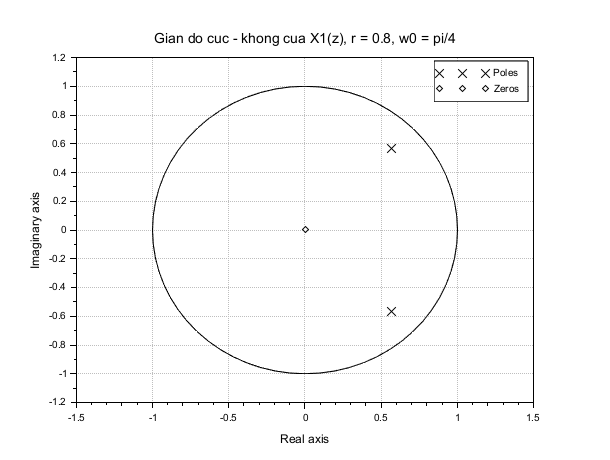
\includegraphics[width=0.65\linewidth]{img/BT3_20_dothi_pz.png}
    \caption{Bài 3.20 -- giản đồ cực -- không của $X_1(z)$ với $r=0{,}8$, $\omega_0=\pi/4$}
\end{figure}
\begin{figure}[H]
    \centering
    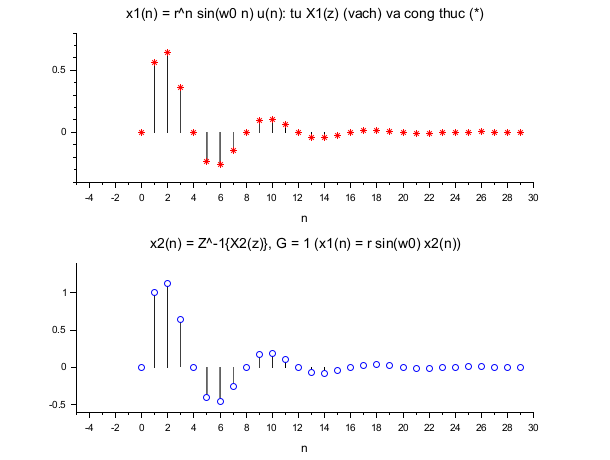
\includegraphics[width=0.8\linewidth]{img/BT3_20_dothi_xn.png}
    \caption{Bài 3.20 -- $x_1(n)$ (trên) và $x_2(n)$ ứng với $G=1$ (dưới): cùng dạng, khác biên độ}
\end{figure}
\begin{figure}[H]
    \centering
    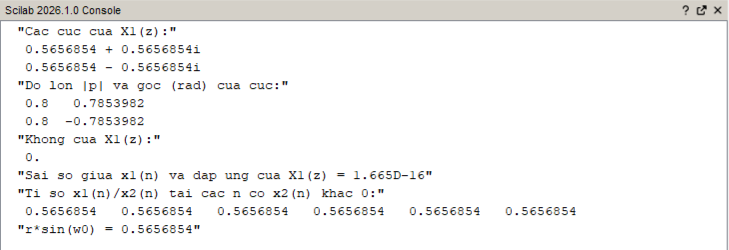
\includegraphics[width=0.75\linewidth]{img/BT3_20_console_crop.png}
    \caption{Bài 3.20 -- ảnh chụp Console}
\end{figure}
\noindent\textbf{Nhận xét:} Scilab cho hai cực $0{,}5657 \pm 0{,}5657j$ có $|p| = 0{,}8 = r$ và góc $\pm 0{,}7854 = \pm\pi/4 = \pm\omega_0$, một không tại $z = 0$, đúng như câu (a). Tỉ số $x_1(n)/x_2(n)$ luôn bằng $0{,}5657 = r\sin\omega_0 = 0{,}8\sin\frac{\pi}{4}$, đúng như kết luận câu (c).

\section*{5. Bàn Luận}
\begin{itemize}
    \item \textbf{ROC quyết định tín hiệu.} Cùng một biểu thức $X(z)$ có thể ứng với nhiều tín hiệu khác nhau (Exercise 3, Bài 3.3 a--b): mỗi vành khuyên giữa các cực cho một tín hiệu. Cực nằm trong đường tròn trong của ROC cho thành phần nhân quả, cực nằm ngoài cho thành phần phản nhân quả.
    \item \textbf{Phương trình sai phân và sơ đồ khối.} Biến đổi $Z$ đưa phương trình sai phân về phương trình đại số để tìm $H(z)$ và $h(n)$ (Exercise 1, 4, 5); biến đổi $Z^{+}$ đưa thêm điều kiện đầu vào để tìm $y_{zi}(n)$. Vị trí cực cho biết ngay tính ổn định: Exercise 4 ổn định (cực $0{,}7$), Exercise 1 biên ổn định (cực $\pm1$), Exercise 5 không ổn định ($|p|=\sqrt3$).
    \item \textbf{Tính chất của biến đổi $Z$} (tích chập, đạo hàm, đảo thời gian, liên hợp, co giãn) giúp tìm biến đổi mà không cần tính trực tiếp tổng chuỗi (Exercise 2, 6; Bài 3.4, 3.7, 3.8, 3.13, 3.19).
    \item \textbf{Khai triển phân thức tối giản} là cách chính để tìm biến đổi ngược. Cần chia đa thức trước khi bậc tử $\ge$ bậc mẫu; cực phức cho thành phần $r^n\cos$, $r^n\sin$, cực kép cho thành phần $(n+1)a^n$. Phép kiểm tra $x(0)=X(\infty)$ giúp phát hiện sai sót khi tính hệ số.
    \item \textbf{Giản đồ cực -- không} xác định $X(z)$ chỉ sai khác một hằng số nhân (Bài 3.20), nên cần thêm hằng số $G$ hoặc một mẫu của tín hiệu (Bài 3.14h).
    \item Một số chỗ trong đề cần đọc lại: ROC của Bài 3.19(b) phải là $|z|>1$ (không phải $|z|>\tfrac12$); ROC của $X_3(z)$ trong Exercise 3 hiểu là $0{,}3<|z|<0{,}5$.
\end{itemize}

\section*{6. Tài Liệu Tham Khảo}
\begin{enumerate}
    \item Tài liệu hướng dẫn thực hành môn học: \textit{DSP2627 - Lab 5}.
    \item J. G. Proakis, D. G. Manolakis, \textit{Digital Signal Processing: Principles, Algorithms, and Applications}, Chương 3: The $z$-Transform and Its Application to the Analysis of LTI Systems.
    \item Mã nguồn Scilab của nhóm trên GitHub:\\ \url{https://github.com/thanhtu988/DSP-lab-5}
\end{enumerate}

\end{document}
